\documentclass[12pt]{article}

\usepackage[shortlabels]{enumitem}
\usepackage{amsmath}

\usepackage{graphicx}
\setkeys{Gin}{width=13cm}

\usepackage{tikz}
\usetikzlibrary{shapes,arrows}

\tikzstyle{block} = [draw, thick, rectangle, minimum height = 3em,
    minimum width = 3em]
\tikzstyle{sum} = [draw, circle, node distance = 2cm]
\tikzstyle{input} = [coordinate]
\tikzstyle{output} = [coordinate]

\title{Feedforward Control Homework 1 \\
  \large National Cheng Kung University, Dept. of Mechanical Engineering}
\date{2019-03-10}
\author{Chien-Ming Chen}

\begin{document}
  \maketitle
  \pagenumbering{arabic}

  \section{Problem 1}
  Consider the model of the flexural stage (Eq. (2) in the attachment by Hector Perez)

  \begin{enumerate}[(a)]
    \item What is the relative degree of the system?

    By definition,

    \begin{equation}
      \text{relative degree} = \text{order of denominator} – \text{order of numerator}
    \end{equation}

    In this case, the transfer function:

    \begin{equation}
      \text{TF} = \frac{11.88 s^4 + 4.977 s^3 + 539.6 s^2 + 129.9 s + 5625}{s^6 + 1.169 s^5 + 50.3 s^4 + 45.94 s^3 + 685.3 s^2 + 391.7 s + 1952}
    \end{equation}

    Where

    \begin{align*}
      \text{order of denominator} &= 6 \\
      \text{order of numerator} &= 4 \\
      \text{relative degree} &= 6 - 4 = 2
    \end{align*}

    \clearpage

    \item Find a state-space model (in control canonical form shown below) of this flexural stage.

    \begin{align*}
      \dot{x} &= Ax + Bu \\
      y &= Cx
    \end{align*}

    Where

    \begin{align*}
      A &= \left(\begin{array}{cccccc} -1.17 & -50.3 & -45.9 & -685.0 & -392.0 & -1966.0\\ 1.0 & 0 & 0 & 0 & 0 & 0\\ 0 & 1.0 & 0 & 0 & 0 & 0\\ 0 & 0 & 1.0 & 0 & 0 & 0\\ 0 & 0 & 0 & 1.0 & 0 & 0\\ 0 & 0 & 0 & 0 & 1.0 & 0 \end{array}\right) \\[2ex]
      B &= \left(\begin{array}{c} 1.0\\ 0\\ 0\\ 0\\ 0\\ 0 \end{array}\right) \\[2ex]
      C &= \left(\begin{array}{cccccc} 0 & 11.9 & 4.98 & 540.0 & 130.0 & 5622.0 \end{array}\right)
    \end{align*}

    \clearpage

    \item Find the inverse system model.

    \begin{align*}
      \begin{split}
      \dot{x}_\text{inv} &= A_\text{inv} x_\text{inv} + B_\text{inv} y^{(r)}_d \\
             &= [A - BK_y] x + [BB_y] y^{(r)}_d \\
             &= \left(\begin{array}{cccccc} -0.419 & -45.4 & -10.9 & -473.0 & -5.68\,{10}^{-14} & 0\\ 1.0 & 0 & 0 & 0 & 0 & 0\\ 0 & 1.0 & 0 & 0 & 0 & 0\\ 0 & 0 & 1.0 & 0 & 0 & 0\\ 0 & 0 & 0 & 1.0 & 0 & 0\\ 0 & 0 & 0 & 0 & 1.0 & 0 \end{array}\right) x + \left(\begin{array}{c} 0.0842\\ 0\\ 0\\ 0\\ 0\\ 0 \end{array}\right) y^{(r)}_d
      \end{split}
      \\[2ex]
      \begin{split}
      u_\text{inv} &= C_\text{inv} x_\text{inv} + D_\text{inv} y^{(r)}_d \\
             &= [-K_y] x + [B_y] y^{(r)}_d \\
             &= [\frac{-CA^r}{CA^{r-1}B}] x + [\frac{1}{CA^{r-1}B}] y^{(r)}_d \\
             &= \left(\begin{array}{cccccc} 0.75 & 4.88 & 35.0 & 212.0 & 392.0 & 1966.0 \end{array}\right) x + 0.0842\ y^{(r)}_d
      \end{split}
    \end{align*}

    \clearpage

    \item Simulate the inverse system model using MATLAB(lsim command) to find the inverse feedforward input. The desired acceleration profile is shown below.
    \item Apply this feedforward input to the system model found in part (b) to verify that the output tracking of y is achieved (use lsim command again).

    \begin{figure}[h]
      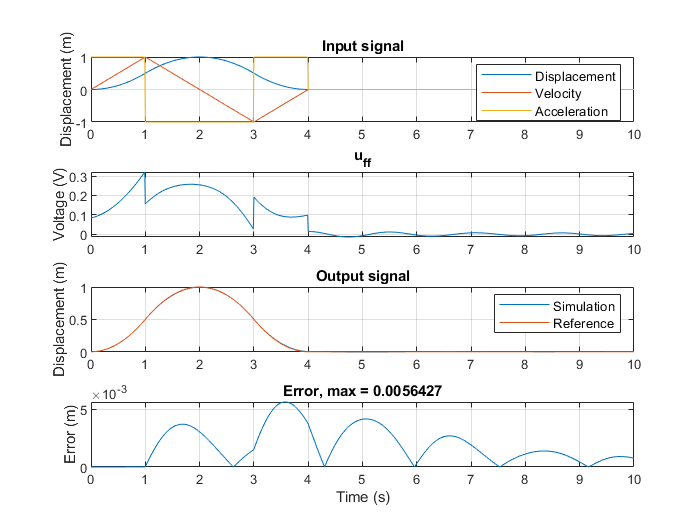
\includegraphics{no_error_ff.png}
      \caption{Simulation result.}
      \centering
    \end{figure}

    \clearpage

    \item Investigate the effect of 5\% variation in the DC gain of the system; in particular simulate the response of the system (using the original inverse input) when the numerator constant 5625 has changed by 5\% and -5\%. What is the maximum error in the output? How could this error be reduced?

    \begin{figure}[h]
      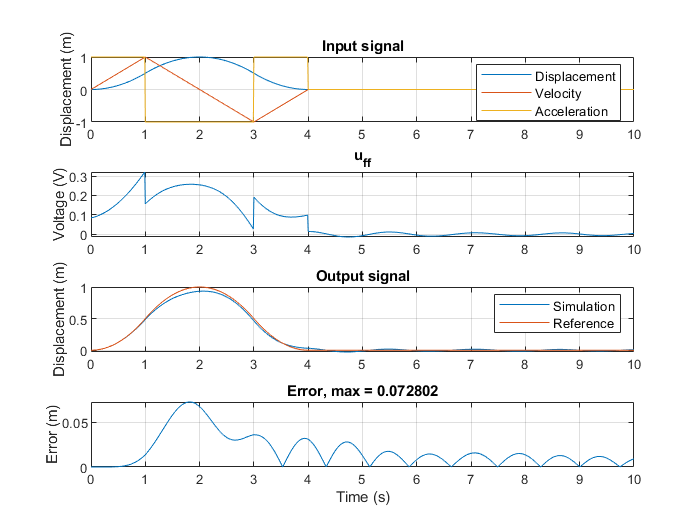
\includegraphics{n5_error_ff.png}
      \caption{System changed by -5\%.}
      \centering
    \end{figure}

    \begin{figure}[h]
      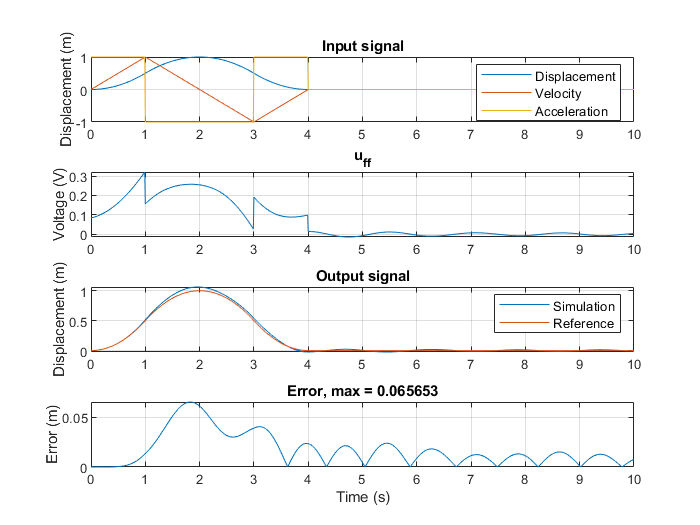
\includegraphics{p5_error_ff.png}
      \caption{System changed by 5\%.}
      \centering
    \end{figure}

    \clearpage

    \item Design a feedback controller and investigate the effect of the 5\% error in the parameter for the closed loop system.

    I design a PID controller for feedback control (Fig \ref{fig:feedbackloop}). From the simulation, we can see that the feedback controller has more robustness than feedforward.

    \begin{figure}[h]
      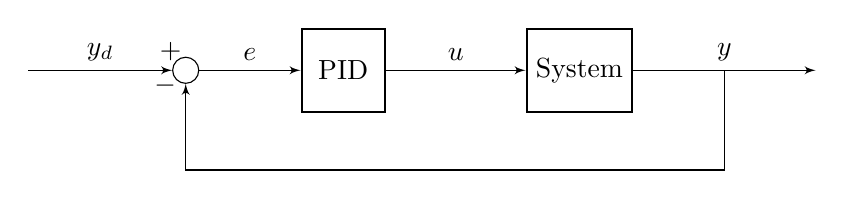
\begin{tikzpicture}[auto, node distance=2cm,>=latex']
          % Place the blocks
          \node [input, name=input] {};
          \node [sum, right of=input] (sum) {};
          \node [block, right of=sum] (controller) {PID};
          \node [block, right of=controller, node distance=3cm] (system) {System};
          \node [output, right of=system, node distance=3cm] (output) {};

          % Connections
          \draw [draw,->] (input) -- node {$y_d$} node[pos=0.99] {$+$} (sum);
          \draw [->] (controller) -- node {$u$} (system);
          \draw [->] (sum) -- node {$e$} (controller);
          \draw [->] (system) -- node [name=y] {$y$}(output);
          \draw [->] (y) -- ++(0,-1.5) -| node[pos=0.99] {$-$} (sum);
      \end{tikzpicture}
      \centering
      \caption{Feedback control loop, where $Kp=30.42, Ki=69.08, Kd=3.349$.}
      \label{fig:feedbackloop}
    \end{figure}

    \begin{figure}[h]
      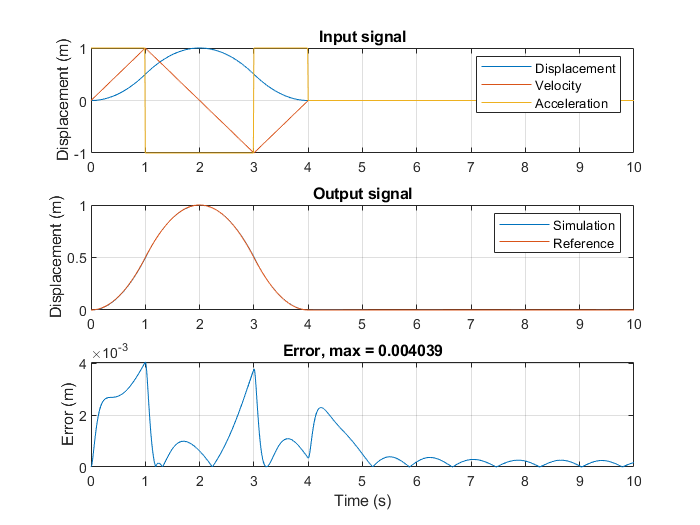
\includegraphics{no_error_fb.png}
      \centering
      \caption{Feedback control without any system variation.}
    \end{figure}

    \begin{figure}[h]
      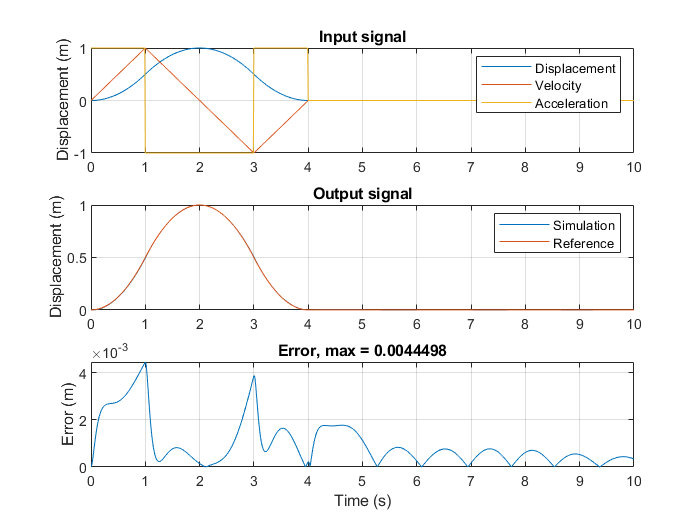
\includegraphics{n5_error_fb.png}
      \centering
      \caption{Feedback control with system changed by -5\%.}
    \end{figure}

    \begin{figure}[h]
      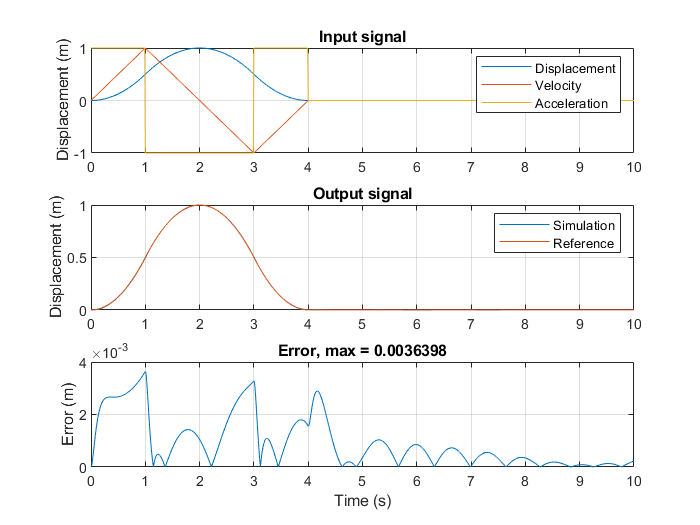
\includegraphics{p5_error_fb.png}
      \centering
      \caption{Feedback control with system changed by 5\%.}
    \end{figure}

    \clearpage

    \item Compare the performance of the system with inverse plus feedback input and without inverse input (i.e., only the feedback input). Compare the tracking error and the magnitude of the total input (feedback and feedforward) applied to this system.

    The inverse plus feedback loop I use shown as Fig \ref{fig:inversefb}. The performance is better than just feedback control even with system variation.

    \begin{figure}[h]
      \begin{tikzpicture}[auto, node distance=2cm,>=latex']
          % Place the blocks
          \node [input, name=input] {};
          \node [sum, right of=input, node distance=2.5cm] (sub) {};
          \node [block, right of=sum] (fbc) {PID};
          \node [block, above of=fbc] (ffc) {Inverse};
          \node [sum, right of=fbc] (sum) {};
          \node [block, right of=sum] (system) {System};
          \node [output, right of=system, node distance=3cm] (output) {};

          % Connections
          \draw [draw,->] (input) -- node [pos=0.1] {$y_d$} node [below, name=r] {} node[pos=0.99] {$+$} (sub);
          \draw [->] (r) |- (ffc);
          \draw [->] (sub) -- node {$e$} (fbc);
          \draw [->] (fbc) -- node {$u_{fb}$} (sum);
          \draw [->] (ffc) -| node {$u_{ff}$} (sum);
          \draw [->] (sum) -- node {$u$} (system);
          \draw [->] (system) -- node [name=y] {$y$}(output);
          \draw [->] (y) -- ++(0,-1.5) -| node[pos=0.99] {$-$} (sub);
      \end{tikzpicture}
      \centering
      \caption{Inverse plus feedback control loop.}
      \label{fig:inversefb}
    \end{figure}

    \begin{figure}[h]
      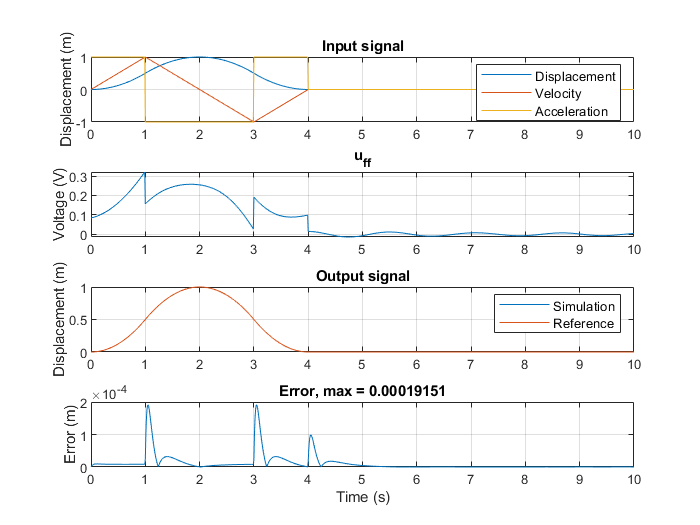
\includegraphics{no_error_ff_fb.png}
      \centering
      \caption{Inverse plus feedback control without any system variation.}
    \end{figure}

    \begin{figure}[h]
      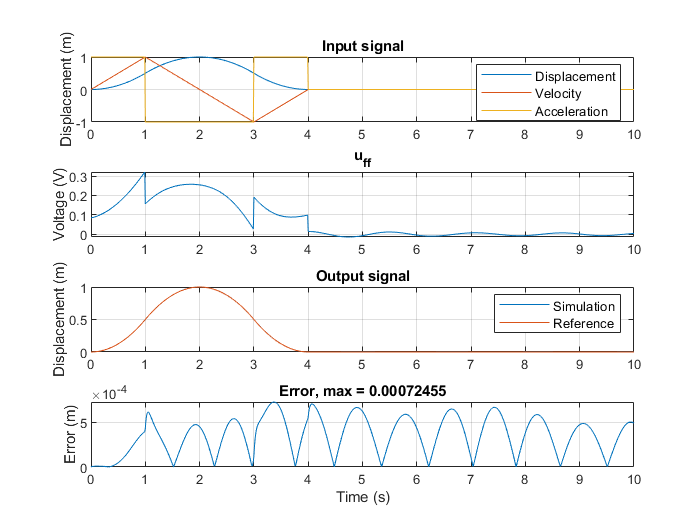
\includegraphics{n5_error_ff_fb.png}
      \centering
      \caption{Inverse plus feedback control with system changed by -5\%.}
    \end{figure}

    \begin{figure}[h]
      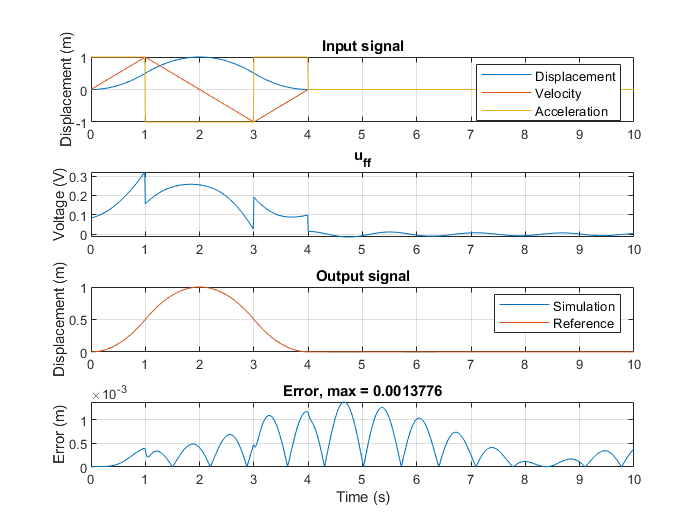
\includegraphics{p5_error_ff_fb.png}
      \centering
      \caption{Inverse plus feedback control with system changed by 5\%.}
    \end{figure}

  \end{enumerate}

  \clearpage

  \section{Problem 2}
  Consider a general transfer function for a linear system with relative degree r=n-m (n greater than or equal to m ).

  \begin{equation}
    G(s) = \frac{b_0 s^m + b_1 s^{m-1} + \dots + b_m}{s^n + a_1 s^{n-1} + \dots + a_n}
  \end{equation}

  Find its description in control canonical form. Show that you need to differentiate the
  output r-times to find the inverse input.

  \hfill

  We can find the control canonical form by the formula provided in previous problem.

  \begin{align}
    \dot{x} &=
    \begin{bmatrix}
    -a_1   & -a_2   & -a_3   & \dots  & -a_{n-1} & -a_n   \\
    1      & 0      & 0      & \dots  & 0        & 0      \\
    0      & 1      & 0      & \dots  & 0        & 0      \\
    \vdots & \vdots & \vdots & \ddots & \vdots   & \vdots \\
    0      & 0      & 0      & \dots  & 0        & 0      \\
    0      & 0      & 0      & \dots  & 1        & 0      \\
    \end{bmatrix} x +
    \begin{bmatrix}
    1 \\ 0 \\ 0 \\ \vdots \\ 0 \\ 0
    \end{bmatrix} u \\
    y &=
    \begin{bmatrix}
    0 & \dots & 0 & b_0 & \dots & b_m
    \end{bmatrix} x
  \end{align}

  Apply the generalized form with k times differentiation to find the inverse input

  \begin{equation}
    u_{ff} = \frac{y^{(k)}_d - CA^kx}{CA^{k-1}B}
    \label{eq:inverseinput}
  \end{equation}

  By equation (\ref{eq:inverseinput}), we can figure out that to get the inverse input, the denominator must not equal to zero, that is

  \begin{equation}
    CA^{k-1}B \neq 0
  \end{equation}

  where

  \begin{align*}
    A &=
    \begin{bmatrix}
    -a_1   & -a_2   & -a_3   & \dots  & -a_{n-1} & -a_n   \\
    1      & 0      & 0      & \dots  & 0        & 0      \\
    0      & 1      & 0      & \dots  & 0        & 0      \\
    \vdots & \vdots & \vdots & \ddots & \vdots   & \vdots \\
    0      & 0      & 0      & \dots  & 0        & 0      \\
    0      & 0      & 0      & \dots  & 1        & 0      \\
    \end{bmatrix}
    \\
    B &=
    \begin{bmatrix}
    1 \\ 0 \\ 0 \\ \vdots \\ 0 \\ 0
    \end{bmatrix}
    \\
    C &=
    \begin{bmatrix}
    0 & \dots & 0 & b_0 & \dots & b_m
    \end{bmatrix}
  \end{align*}

  firstly, by expanding $A^{k-1}B$, we get

  \begin{equation}
    \begin{split}
      A^{k-1}B &=
      \begin{bmatrix}
      e_{11} & e_{12} & e_{13} & \dots & e_{1(n-1)} & e_{1n}   \\
      e_{21} & e_{22} & e_{23} & \dots  & e_{2(n-1)} & e_{2n} \\
      \vdots & \vdots & \vdots & \ddots & \vdots   & \vdots \\
      e_{(k-1)1} & e_{(k-1)2} & e_{(k-1)3} & \dots  & e_{(k-1)(n-1)} & e_{(k-1)n} \\
             &        &        & \dots  & 0        & 0      \\
             & I_{n-(k-1)} &        & \ddots  & \vdots        & \vdots      \\
             &        &        & \dots  & 0        & 0      \\
      \end{bmatrix}
      \begin{bmatrix}
      1 \\ 0 \\ 0 \\ \vdots \\ 0 \\ 0
      \end{bmatrix} \\
      &=
      \begin{bmatrix}
      e_{11} \\ e_{21} \\ \vdots \\ e_{(k-1)1} \\ 1 \\ \vdots \\ 0
      \end{bmatrix}
    \end{split}
  \end{equation}

  We found that if $k$ less than $(n-m)$, $CA^{k-1}B$ will derive to $0$, which means that to get non-zero $CA^{k-1}B$, $k$ must larger or equal to $(n-m)$, which is the relative order.

\end{document}
